%%%%%%%%%%%%%%%%%%%%%%%%%%%%%%%%%%%%%%%%
%% Slides : Bayes basics ("bayesics") %%
%%%%%%%%%%%%%%%%%%%%%%%%%%%%%%%%%%%%%%%%

%% PREAMBLE
%% Define document class and basic options
\documentclass{beamer}
%\setlength{\parindent}{0pt}

%% Load packages
\usepackage{palatino}
\usepackage{amsfonts}
\usepackage{amsmath}
%\usepackage{url}
\usepackage{hyperref}
%\usepackage{listings}
\usepackage{verbatim}
\usepackage[utf8]{inputenc} %% For french
\usepackage{tikz} %% For drawing (eg, Venn diagrams)

\hypersetup{
	colorlinks=true,
	linkcolor=blue,
	citecolor=red,
	filecolor=blue,
	urlcolor=blue
}

\usetheme{Madrid}

%% Basic info
\title{Introduction à la pensé et aux méthodes bayésiennes}
%\subtitle{}
\author{Roy Nitulescu\inst{1}}

\institute
{
    \inst{1}%
    CITADEL\\
    CR-CHUM
}

\date[UdeM, Sept. 22, 2021]{Université de Montréal, Sept. 22, 2021}

\AtBeginSection[]
{
    \begin{frame}
        \frametitle{Table des matières}
        \tableofcontents[currentsection]
    \end{frame}
}

\AtBeginSubsection[]
{
    \begin{frame}
        \frametitle{Table des matières}
        \tableofcontents[currentsubsection]
    \end{frame}
}


%% BEGIN DOCUMENT
\begin{document}

%%%%
%% Slides
%%%%

\frame{\titlepage}

\begin{frame}
    \frametitle{Épigraphe}
    ``La probabilité est le concept le plus important de la science moderne,
    d'autant plus que personne n'a la moindre idée de ce qu'elle signifie.'' -- Bertrand Russell, 1929
\end{frame}


\begin{frame}
    \frametitle{Préambule}
%    \begin{itemize}
%      \item This 3-hour lecture will be broken down into 3 modules
%      \item Each module will last 50 minutes
%      \begin{itemize}
%        \item 30 minutes of lecture time
%        \item 10 minutes for exercises
%        \item 10 minutes for discussing the exercises
%      \end{itemize}
%      \item There will be two 15-minute breaks between the modules
%      \item I expect that all students have already installed R on their computer and tested that it works
%    \end{itemize}
    
%    \vfill
    
    Le code source pour cette présentation ce trouve içi:\\
    \url{https://github.com/rnitulescu/bayesics}
\end{frame}


\begin{frame}
    \frametitle{Table des matières}
    \tableofcontents
\end{frame}


%%%%
%% Motivation
%%%%

\section{Motivation}

\begin{frame}
    \frametitle{La dualité du concept de probabilité}

    De par son origine, le concept à une \textbf{dualité}\footnote{
    Hacking, Ian (1975). \emph{The emergence of probability:
    A philosophical study of early ideas about probability,
    induction and statistical inference}. Cambridge University Press.
    }

    \pause

    \vfill

    \begin{enumerate}
      \item \textbf{Aléatoire}
        \begin{itemize}
          \item Fréquence (la limite d'une fréquence relative dans une séquence infinie)
          \item Propensité (une propriété intrinsèque d'objets ou de situations)
        \end{itemize}

      \pause

      \item \textbf{Épistémique}
        \begin{itemize}
          \item Logique (le degré de soutien ou de confirmation qu'un élément d'évidence confère à une hypothèse donnée)
          \item Subjectif (le degré de croyance subjectif)
        \end{itemize}
    \end{enumerate}    
\end{frame}


\begin{frame}
    \frametitle{Plusieurs interprétations}
    Donc, plusieurs \textbf{interprétations} de la probabilité ont été proposées. Mais, comment les évaluons-nous?
    
    \pause

    \vfill

    Des \textbf{critères} d’évaluation proposés: ``admissibility'', ``ascertainability'', ``applicability''\footnote{
    Salmon, W. C. (1967). \emph{The foundations of scientific inference}.
    University of Pittsburgh Press.
    }

    \pause

    \vfill

    Mais \textbf{aucune} des interprétations ne répond à tous ces critères.

    \pause

    \vfill

    Pour plus de détails, voir aussi:
    \href{https://plato.stanford.edu/entries/probability-interpret/}{https://plato.stanford.edu}
\end{frame}


\begin{frame}
    \frametitle{Plusieurs systèmes de probabilité}
    Plusieurs \textbf{systèmes} axiomatiques de probabilité ont été développés.

    \begin{itemize}
      \item Kolmogorov (fréquence)
      \item Carnap (logique)
      \item De Finetti (subjectif/personnaliste)
    \end{itemize}

    \pause

    \vfill

    En pratique, ces systèmes sont souvent plus semblables que différents.

    \pause

    \vfill

    Il y a même le \textbf{Théorème de Bernstein-von Mises} qui relient le système fréquentiste
    d’inférence au système bayésien (en bref, sous certaines hypothèses, asymptotiquement,
    les intervalles de confiances sont équivalents aux intervalles crédibles bayésiennes).
    \footnote{
      \url{https://en.wikipedia.org/wiki/Bernstein-von_Mises_theorem}
    }
\end{frame}


\begin{frame}
    \frametitle{Soyons pragmatiques}
    Gardant en tête tous ces problèmes philosophiques et l’impossibilité de faire un choix absolument objectif,
    pourquoi ne pas avoir une approche plutôt axé sur ce qui est \textbf{pratique}?

    \pause

    \vfill

    En pratique, les méthodes bayésiennes nous fournissent souvent plus \textbf{d’outils} et plus de
    \textbf{flexibilité} que ceux Fréquentistes, et tous cela dans le cadre d’une méthodologie \textbf{cohérente}
    basé sur des principes fondamentaux de la théorie de la probabilité.

    \pause
    
    \vfill

    Elles nous permettent même \textbf{d’intégrer} des nouvelles données avec \textbf{nos connaissances déjà acquises} 
    dans le but d’avancer nos connaissances.
\end{frame}


\section{Théorie de la probabilité (révision)}

\begin{frame}
    \frametitle{Propriétés de la probabilité}
    \[p(A^c) = 1 - p(A), \,\,\, \textrm{puisque} \,\,\, A \cup A^c = S\]
    \begin{figure}
      \centering
      \scalebox{1}{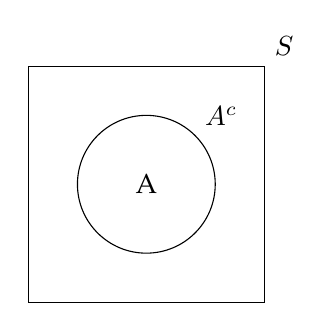
\begin{tikzpicture}
    % Sample space
    \node [draw,
    rectangle,
    minimum size =3cm,
    label={45:$S$}] (S) at (0,0){};

    % Set A
    \node [draw,
    circle,
    minimum size =1.75cm, text centered,
    label={45:$A^c$}] (A) at (0,0){A};
\end{tikzpicture}

}
      \caption{Diagramme de Venn représentant la négation (complément)}
    \end{figure}
\end{frame}


\begin{frame}
    \frametitle{Propriétés de la probabilité}
    \[p(A \cup B) = p(A) + p(B) - p(A \cap B)\]\footnote{
        Si $A$ et $B$ sont mutuellement exclusifs, $p(A \cap B) = 0$
    }
    \begin{figure}
      \centering
      \scalebox{1}{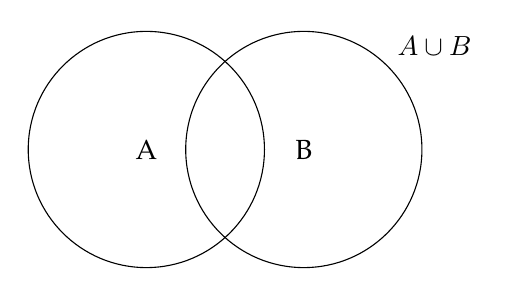
\begin{tikzpicture}
    % Set A
    \node [draw,
    circle,
    minimum size =3cm, text centered] (A) at (0,0){A};

    % Set B
    \node [draw,
    circle,
    minimum size =3cm, text centered,
    label={45:$A \cup B$}] (B) at (2,0){B};
\end{tikzpicture}

}
      \caption{Diagramme de Venn représentant $p(A \cup B)$}
    \end{figure}    
\end{frame}


\begin{frame}
    \frametitle{Probabilité d'intersection et probabilité conditionnelle}
    \[p(A \cap B) = p(A | B) \, p(B) \,\,\, \textrm{Donc,} \,\,\, p(A | B) = \frac{p(A \cap B)}{p(B)}\]

    \begin{figure}
      \centering
      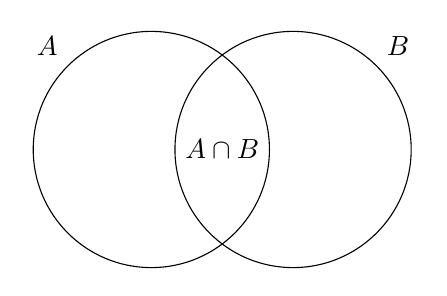
\begin{tikzpicture}
    % Set A
    \node [draw,
    circle,
    minimum size =3cm,
    label={135:$A$}] (A) at (0,0){};

    % Set B
    \node [draw,
    circle,
    minimum size =3cm,
    label={45:$B$}] (B) at (1.8,0){};

    % Set intersection label
    \node at (0.9,0) {$A\cap B$};
\end{tikzpicture}


      \caption{Diagramme de Venn représentant $p(A \cap B)$}
    \end{figure}
\end{frame}


\begin{frame}
    \frametitle{Loi de probabilité totale}

    \[p(E) = p(E \cap H) + p(E \cap H^c)\]
    \[ = p(E | H) \, p(H) + p(E | H^c) \, p(H^c)\]

    \begin{figure}
      \centering
      \begin{tikzpicture}
    % Hypothesis is true
    \node [draw,
    rectangle,
    minimum size =3cm,
    label={135:$H$}] (H) at (-1.5,0){};

    % Hypothesis is false
    \node [draw,
    rectangle,
    minimum size =3cm,
    label={45:$H^c$}] (Hc) at (1.5,0){};

    % Set E for evidence is true
    \node [draw,
    circle,
    minimum size =2.5cm,
    label={145:$E$}] (E) at (0,0){};
\end{tikzpicture}


      \caption{Diagramme de Venn représentant loi de probabilité totale}
    \end{figure}
\end{frame}


%%%%
%% Intuition
%%%%

\section{Intuition}

\begin{frame}
    \frametitle{Exemple: diagnostic de maladie\footnote{
        Emprunté et modifié d'un exemple pris dans: Devlin, Keith (2010).
        \emph{The unfinished game: Pascal, Fermat, and the seventeenth-century letter that made the world modern.}
        Basic Books, pp 139-142.
    }}
    Supposons que vous avez reçu un résultat positif pour un test diagnostic d'une maladie rare.
    Quelle est la probabilité que vous avez cette maladie, conditionnellement sur le résultat du test?

    \pause

    \vfill

    Voici les faits:
    \begin{itemize}
      \item Prévalence: Parmi \textbf{10,000} individus, \textbf{100} ont la maladie (donc, \textbf{9,900} ne l'ont pas)
      \pause
      \item Sensibilité du test: Parmi les \textbf{100} malades,
            \textbf{95} reçoivent un diagnostic positif (donc, \textbf{5} faux négatifs)
      \pause
      \item Spécificité du test: Parmi les \textbf{9,900} en santé,
            \textbf{7,821} reçoivent un diagnostic négatif (donc, \textbf{2,079} faux positifs)
    \end{itemize}
\end{frame}


\begin{frame}
    \frametitle{Exemple: diagnostic de maladie}
    \begin{figure}
      \centering
      \scalebox{0.75}{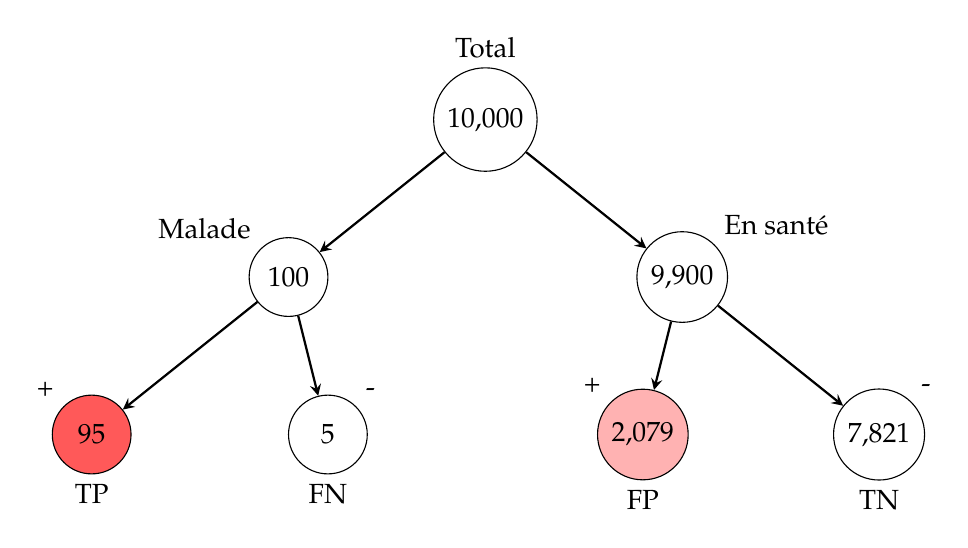
\begin{tikzpicture}
    \tikzstyle{arrow} = [thick,->,>=stealth]
    % Top bubble
    \node [draw, circle, minimum size=1cm, text centered, label={90:Total}] (Top) at (0,5) {10,000};

    % Lower left bubble
    \node [draw, circle, minimum size=1cm, text centered, label={135:Malade}] (Diseased) at (-2.5,3) {100};
    \draw [arrow] (Top) -- (Diseased);

    % Lower right bubble
    \node [draw, circle, minimum size=1cm, text centered, label={45:En santé}] (NonDiseased) at (2.5,3) {9,900};
    \draw [arrow] (Top) -- (NonDiseased);

    % Bottom extreme left
    \node [draw, circle, minimum size=1cm, text centered, label={135:+}, label={-90:TP}, fill=red!65] (TP) at (-5,1) {95};
    \draw [arrow] (Diseased) -- (TP);

    % Bottom mid left
    \node [draw, circle, minimum size=1cm, text centered, label={45:-}, label={-90:FN}] (FN) at (-2,1) {5};
    \draw [arrow] (Diseased) -- (FN);

    % Bottom mid right
    \node [draw, circle, minimum size=1cm, text centered, label={135:+}, label={-90:FP}, fill=red!30] (FP) at (2,1) {2,079};
    \draw [arrow] (NonDiseased) -- (FP);

    % Bottom extreme right
    \node [draw, circle, minimum size=1cm, text centered, label={45:-}, label={-90:TN}] (TN) at (5,1) {7,821};
    \draw [arrow] (NonDiseased) -- (TN);
\end{tikzpicture}

}
    \end{figure}

    \pause

    La proportion des patients avec un test positif qui sont véritablement malades est de
    \[\frac{95}{95 + 2079} = 0.044 .\]
\end{frame}


\begin{frame}
    \frametitle{Exemple: diagnostic de maladie (en probabilités)}
    \begin{figure}
      \centering
      \scalebox{0.65}{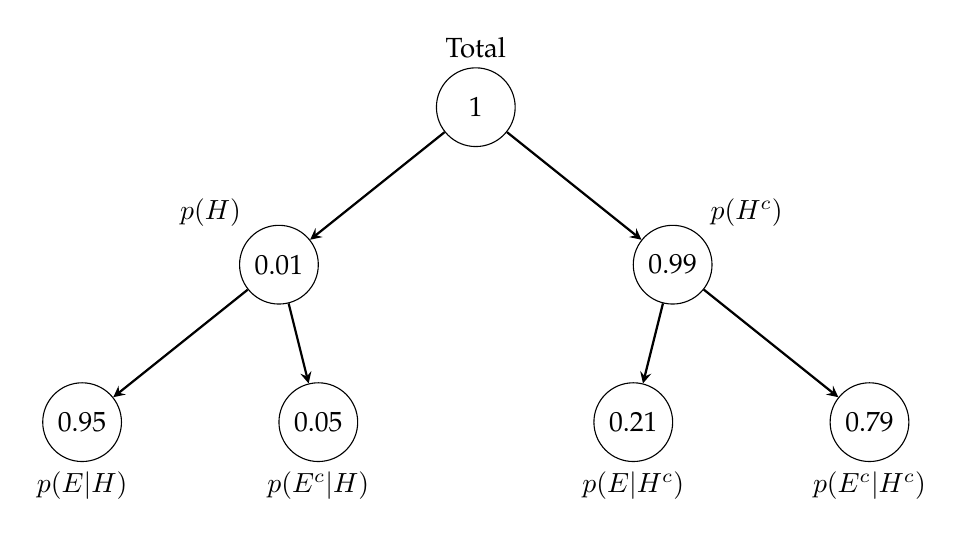
\begin{tikzpicture}
    \tikzstyle{arrow} = [thick,->,>=stealth]
    % Top bubble
    \node [draw, circle, minimum size=1cm, text centered, label={90:Total}] (Top) at (0,5) {1};

    % Lower left bubble
    \node [draw, circle, minimum size=1cm, text centered, label={135:$p(H)$}] (Diseased) at (-2.5,3) {0.01};
    \draw [arrow] (Top) -- (Diseased);

    % Lower right bubble
    \node [draw, circle, minimum size=1cm, text centered, label={45:$p(H^c)$}] (NonDiseased) at (2.5,3) {0.99};
    \draw [arrow] (Top) -- (NonDiseased);

    % Bottom extreme left
    \node [draw, circle, minimum size=1cm, text centered, label={-90:$p(E | H)$}] (TP) at (-5,1) {0.95};
    \draw [arrow] (Diseased) -- (TP);

    % Bottom mid left
    \node [draw, circle, minimum size=1cm, text centered, label={-90:$p(E^c | H)$}] (FN) at (-2,1) {0.05};
    \draw [arrow] (Diseased) -- (FN);

    % Bottom mid right
    \node [draw, circle, minimum size=1cm, text centered, label={-90:$p(E | H^c)$}] (FP) at (2,1) {0.21};
    \draw [arrow] (NonDiseased) -- (FP);

    % Bottom extreme right
    \node [draw, circle, minimum size=1cm, text centered, label={-90:$p(E^c | H^c)$}] (TN) at (5,1) {0.79};
    \draw [arrow] (NonDiseased) -- (TN);
\end{tikzpicture}

}
    \end{figure}

    \pause

    Si ont suit l'arbre de façon analogique:
    \[p(H | E) = \frac{(0.95)(0.01)}{(0.95)(0.01) + (0.21)(0.99)}\]
    \pause
    \[ = \frac{p(E | H) \, p(H)}{p(E | H) \, p(H) + p(E | H^c) \, p(H^c)} = \frac{p(E | H) \, p(H)}{p(E)}\]
\end{frame}

%% Add Krushchke like example??


%%%%
%% Théorie
%%%%

\section{Théorie bayésienne}

%% formally present bayes theoerem even tough we sort of saw it informally in above section
%% the big step here is De Finetti's theorem, since it allows us to do some cool modeling, etc.
%% Present the model of the mean with know or unknown variance, etc. (do we need to go that far??)

\begin{frame}
    \frametitle{Le théorème de Bayes (probabilités discrètes)}
    Le théorème suit directement de la définition de probabilité conditionnelle:

    \pause

    \[p(A \cap B) =  p(A | B) \, p(B) \,\,\, \pause \textrm{ et } \,\,\, p(B \cap A) =  p(B | A) \, p(A)\]
    \pause
    \[\textrm{Et puisque } \,\,\, p(A \cap B) = p(B \cap A)\]
    \pause
    \[\textrm{Il suit que } \,\,\, p(A | B) \, p(B) = p(B | A) \, p(A)\]
    \pause
    \[\textrm{Donc } \,\,\, p(A | B) = \frac{p(B | A) \, p(A)}{p(B)}\]
    
    Voilà!
\end{frame}


\begin{frame}
    \frametitle{Le théorème de Bayes (probabilités continues)}
    Le théorème suit directement de la définition de la densité conditionnelle:

    \pause

    \[p_{X|Y}(x|y) = \frac{p_{X,Y}(x,y)}{p_Y(y)} \,\,\, \pause \textrm{ et }\]
    \[p_{Y|X}(y|x) = \frac{p_{X,Y}(x,y)}{p_X(x)}\]
    \pause
    \[\textrm{Donc, il suit que } \,\,\, p_{X|Y}(x|y) \, p_Y(y) = p_{Y|X}(y|x) \, p_X(x)\]
    \pause
    \[\textrm{Ce qui implique que } \,\,\, p_{X|Y}(x|y) = \frac{p_{Y|X}(y|x) \, p_X(x)}{p_Y(y)}\]

    Voilà!
\end{frame}


\begin{frame}
    \frametitle{Comment appliquons-nous cela?}
    Comment faisons-nous pour appliquer ce théorème à des problèmes 
    d'inférence probabilistes?

    \pause

    \vfill

    Supposons qu'il y à une issue, $\boldsymbol{y}$, qui suit une loi, $\boldsymbol{p(y)}$.

    \pause

    \vfill

    Et supposons qu'on pense qu'il y a de l'incertitude à propos d'un paramètre, $\boldsymbol{\theta}$,
    de cette loi et que nous sommes intéressés à estimer cette incertitude à partir d'observations de $\boldsymbol{y}$.

    \pause

    \vfill
    
    De la perspective mathématique, il n'est pas nécessairement faux d'écrire
    \[p(y) = \int_{\Theta} p(y, \theta) \, d\theta = \int_{\Theta} p(y | \theta) \, p(\theta) \, d\theta.\]

    %% Show a naive attempt and how it brings up the question:
    %% where do these probs, parameters, priors even come from?!?
    %% Enter De Finetti's theorem which justifies it all with the
    %% assumption of exchangeability (or conditional of some factors, etc.)
\end{frame}


\begin{frame}
    \frametitle{Comment appliquons-nous cela?}
    Donc, en principe, qu'est ce qui nous empêche d'applique le théorème de Bayes
    pour estimer cette incertitude à propos de $\boldsymbol{\theta}$ après avoir
    observé $\boldsymbol{y}$?
    \[p(\theta | y) = \frac{p(y | \theta) \, p(\theta)}{p(y)} =
      \frac{p(y | \theta) \, p(\theta)}{\int_{\Theta} p(y | \theta) \, p(\theta) \, d\theta} \, \, \, \textrm{?}\]
    
    \pause

    \vfill

    \textbf{Le problème:}
    \begin{itemize}
      \item Comment sais-on qu'un modèle paramétrique, $\boldsymbol{p(y | \theta)}$, existe?
      \pause
      \item Comment sais-on qu'une probabilité \emph{a priori}, $\boldsymbol{p(\theta)}$, existe?
    \end{itemize}

    \vfill

    \pause

    \textbf{Réponse:} Le théorème de De Finetti. \pause Mais avant, une définition...
\end{frame}

%% NEED TO TRANSLATE NEXT 2-3 SLIDES TO FRENCH
%% Spell check with: hunspell -l -t -d fr_CA slides.tex (take out -l for interactive, check man 1st)

\begin{frame}
    \frametitle{L'échangeabilité\footnote{
        Bernardo, J. M. (1996).
        The concept of exchangeability and its applications.
        \emph{Far East Journal of Mathematical Sciences}, \emph{4}, 111-122.
    }}
    \textbf{Définition}

    \pause

    \vfill

    Une séquence (finie ou infinie) de variables aléatoires, $\boldsymbol{\{x_1, x_2, \ldots\}}$,
    est dite \emph{échangeable} si pour tout sous-ensemble finie de la séquence
    et pour toutes permutations, $\boldsymbol{\pi}$, définie sur l'ensemble $\boldsymbol{\{1, \ldots, n\}}$
    \[p(x_1, \ldots, x_n) = p(x_{\pi(1)}, \ldots, x_{\pi(n)}).\]

%    A (finite or infinite) sequence of random variables, $\boldsymbol{\{x_1, x_2, \ldots\}}$,
%    is said to be \emph{exchangeable} if for any finite subset of the sequence
%    and for all permutations, $\boldsymbol{\pi}$, defined over the set $\boldsymbol{\{1, \ldots, n\}}$
%    \[p(x_1, \ldots, x_n) = p(x_{\pi(1)}, \ldots, x_{\pi(n)}).\]

    \pause

    \vfill

    Essentiellement, ceci est une vague hypothèse\footnote{
    Peut être supposé conditionnellement sur d'autres variables également.} de symétrie \pause
    De plus, cette hypothèse est plus faible que \emph{indépendant et identiquement distribué} (i.i.d.). \pause
    Tandis que i.i.d. implique l'échangeabilité, l'inverse n'est pas vraie!
\end{frame}


\begin{frame}
    \frametitle{Le théorème de De Finetti (cité en Anglais)}

    \vfill
    
    \textbf{De Finetti's representation theorem (from Bernardo, 1996)}\footnote{
    Notez que de par ce théorème, l'échangeabilité et i.i.d \emph{conditionnelle} sont équivalents.}

    \pause

    \vfill

%% The french is too gross for this theorem...
%    Si $\boldsymbol{\{x_1, x_2, \ldots\}}$ est une séquence échangeable de quantités aléatroires (à valeurs réels),
%    \emph{il existe} une \emph{modèle} paramétrique, $\boldsymbol{p(x | \theta)}$, labelled by some
%    parameter $\boldsymbol{\theta \in \Theta}$ which is the limit (as $\boldsymbol{n \to \infty}$)
%    of some function of the $\boldsymbol{x_i}$'s, and \emph{there exists} a probability distribution
%    for $\boldsymbol{\theta}$, with density $\boldsymbol{p(\theta)}$, such that

    If $\boldsymbol{\{x_1, x_2, \ldots\}}$ is an exchangeable sequence of real-valued random quantities, \pause
    then \emph{there exists} a parametric \emph{model}, $\boldsymbol{p(x | \theta)}$, labelled by some
    parameter $\boldsymbol{\theta \in \Theta}$ which is the limit (as $\boldsymbol{n \to \infty}$)
    of some function of the $\boldsymbol{x_i}$'s, \pause and \emph{there exists} a probability distribution
    for $\boldsymbol{\theta}$, with density $\boldsymbol{p(\theta)}$, such that \pause

    \[p(x_1, \ldots, x_n) = \int_{\Theta} \prod_{i = 1}^{n} p(x_i | \theta) \, p(\theta) \, d\theta.\]
\end{frame}


\begin{frame}
    \frametitle{Le théorème de De Finetti}
    Ça ressemble pas mal à ce qu'on avais plus tôt, n'est-ce pas? (Retournons voir en arrière...)

    \pause

    \vfill

    \begin{itemize}
      \item Donc, sous l'hypothèse d'échangeabilité (conditionnelle ou inconditionnelle), ce théorème justifie
            qu'on utilise un modèle paramétrique et des probabilités \emph{a priori}
      \pause
      \item Bien entendu le problème de \emph{bien spécifier} le modèle ne disparait pas par magie
      \pause
      \item Mais, c'est un début
    \end{itemize}
\end{frame}




%%%%
%% Applications
%%%%

\section{Applications}

%% the bulk of content
%% have the sex ratio example from Aki Vehtari, etc.


%%%%
%% Conclusion
%%%%

\section{Conclusion}

\begin{frame}
    \frametitle{Références et lectures suggérées}

    Philosophie:
    \begin{itemize}
      \item Hacking, I. (1975). \emph{The emergence of probability:
            A philosophical study of early ideas about probability,
            induction and statistical inference}. Cambridge University Press.
      \item Salmon, W. C. (1967). \emph{The foundations of scientific inference}.
            University of Pittsburgh Press.
    \end{itemize}

    Méthodes bayésiennes:
    \begin{itemize}
      \item Kruschke, J. K. (2013). Bayesian estimation supersedes the t test.
            \emph{Journal of Experimental Psychology: General}, \emph{142}(2), 573.
      \item Kruschke, J. K., \& Vanpaemel, W. (2015). Bayesian estimation in hierarchical models.
            \emph{The Oxford handbook of computational and mathematical psychology, 279}.
      \item Kruschke, J. K.(2015). \emph{Doing Bayesian data analysis: A tutorial with R, JAGS, and Stan}.
            Academic Press.
      \item Gelman, A., Carlin, J. B., Stern, H. S., \& Rubin, D. B. (1995).
            \emph{Bayesian data analysis}. Chapman and Hall/CRC.
    \end{itemize}
\end{frame}


%% END DOCUMENT
\end{document}

